\documentclass{article}
\usepackage[utf8]{inputenc}
\usepackage{amsmath}
\usepackage{graphicx}

\title{Report 1: Gradient Descent}
\author{Dang Vu Son Tung}
\date{29/04/2025}

\begin{document}

\maketitle

\section*{Objective}
The goal of this lab is to implement the gradient descent algorithm from scratch to find the minimum of a given function. The example function used is: 

\[
f(x) = x^2
\]

\section*{Method}
I used gradient descent with the following update rule:

\[
x = x - r \cdot f'(x)
\]

Where \( r \) is the learning rate, and \( f'(x) = 2x \) is the derivative of \( f(x) = x^2 \).

The experiment starts from \( x_0 = 10 \) and runs for 10 iterations.

\section*{Results (Learning rate = 0.1)}

\begin{center}
\begin{tabular}{|c|c|c|}
\hline
Iteration & x & f(x) \\
\hline
1 & 10.0000 & 100.0000 \\
2 & 8.0000 & 64.0000 \\
3 & 6.4000 & 40.9600 \\
4 & 5.1200 & 26.2144 \\
5 & 4.0960 & 16.7772 \\
6 & 3.2768 & 10.7374 \\
7 & 2.6214 & 7.0719 \\
8 & 2.0972 & 4.4000 \\
9 & 1.6777 & 2.8136 \\
10 & 1.3422 & 1.8010 \\
\hline
\end{tabular}
\end{center}

\section*{Comparison of Learning Rates}

To analyze the effect of different learning rates, I tested three values: \( r = 0.01 \), \( r = 0.1 \), and \( r = 0.5 \). The final results after 10 steps are:

\begin{center}
\begin{tabular}{|c|c|c|}
\hline
Learning Rate & Final x & Final f(x) \\
\hline
0.01 & 8.3375 & 69.5135 \\
0.10 & 1.3422 & 1.8014 \\
0.50 & 0.0000 & 0.0000 \\
\hline
\end{tabular}
\end{center}

\begin{center}
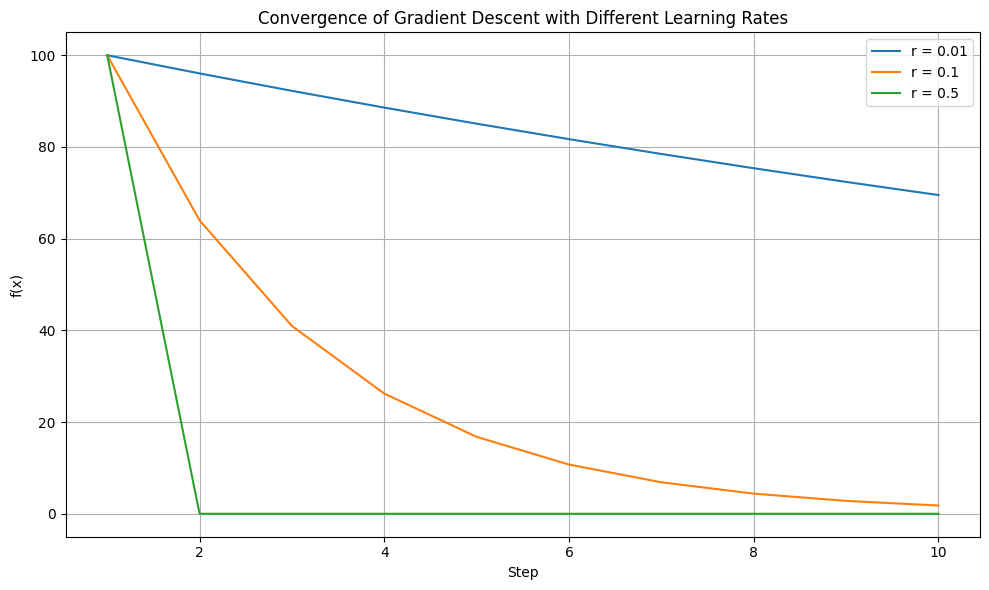
\includegraphics[width=0.85\textwidth]{plot.png}
\end{center}

\textbf{Note:} The graph above shows how the function value \( f(x) \) decreases over iterations for each learning rate.

\section*{Discussion}

The value of \( f(x) \) consistently decreases with each iteration, confirming that gradient descent works well on convex functions like \( f(x) = x^2 \).

From the comparison:
\begin{itemize}
    \item \( r = 0.01 \): very slow convergence, still far from minimum after 10 steps.
    \item \( r = 0.10 \): good balance between speed and stability.
    \item \( r = 0.50 \): converges fastest, but in more complex functions it may overshoot or diverge.
\end{itemize}

Choosing the optimal learning rate depends on the specific problem. A moderate value like 0.1 is often a good default.

\section*{Conclusion}

Gradient descent successfully found the minimum of \( f(x) = x^2 \) in different settings. The experiment helped me understand how learning rate influences convergence and why tuning it is important.

\end{document}
